%
% File acl2017.tex
%
%% Based on the style files for ACL-2015, with some improvements
%%  taken from the NAACL-2016 style
%% Based on the style files for ACL-2014, which were, in turn,
%% based on ACL-2013, ACL-2012, ACL-2011, ACL-2010, ACL-IJCNLP-2009,
%% EACL-2009, IJCNLP-2008...
%% Based on the style files for EACL 2006 by 
%%e.agirre@ehu.es or Sergi.Balari@uab.es
%% and that of ACL 08 by Joakim Nivre and Noah Smith

\documentclass[11pt,a4paper]{article}
\usepackage[hyperref]{acl2017}
\usepackage{times}
\usepackage{latexsym}
\usepackage{graphicx,psfrag,epsf}
\usepackage{multirow}

\usepackage{url}

\aclfinalcopy % Uncomment this line for the final submission
%\def\aclpaperid{***} %  Enter the acl Paper ID here

%\setlength\titlebox{5cm}
% You can expand the titlebox if you need extra space
% to show all the authors. Please do not make the titlebox
% smaller than 5cm (the original size); we will check this
% in the camera-ready version and ask you to change it back.

\newcommand\BibTeX{B{\sc ib}\TeX}
\newcommand{\specialcell}[2][c]{%
	\begin{tabular}[#1]{@{}c@{}}#2\end{tabular}}

\title{Improving Semantic Question Matching of Quora Dataset by Feature-rich Classifiers and LSTM Encoders}

\author{Tian Chen \\
	Department of Statistics \\
	University of California, Irvine \\
	{\tt tianc2@uci.edu} 
	 \\\And
	Huan Chen \\
	School of Information and Computer Science \\
	University of California, Irvine \\
	{\tt huanc3@uci.edu} \\
  }

\date{}

\begin{document}
\maketitle
\begin{abstract}
In this paper, we are interested in identifying duplicate questions for a Quora question pair dataset. Previous work are mostly developed on small dataset (e.g. 5k pairs). We thus propose to use two data-intensive models for this task: a feature-rich classifier model and a neural network model using LSTM sentence embedding. They are both proposed by Bowman  \cite{bowman2015large} and are developed on a large corpus: Stanford Natural Language Inference (SNLI). We evaluate these two methods on a subset of Quora's dataset and showed that they both outperforms the baseline method. Overall, the feature-rich classifier based on lexicalized features achieves the best performance.
\end{abstract}

\section{Introduction}
Recently, Quora released over 400,000 pairs of potential duplicate questions on Kaggle and competitors are required to identify the actual duplicate pairs. That being said, given two sentences, we have to determine if they have the same meaning. This is the problem of paraphrase identification. In this paper, we name the task as semantic question matching, since the sentences are all questions. This is an important NLP task in many applications. As for on-line Question-Answering (QA) communities such as Quora and Stack-Overflow, it helps to maintain their high quality content. It also helps prevent spam users from duplicating the questions and answers from existing ones to gain reputation. In terms of information retrieval, with text-pair identification, query refinement can be conducted to perform targeted searching, etc. 

In the Quora dataset, a sentence pair of the input data set of this task can be "How do I read and find my YouTube comments?" and "How can I see all my Youtube comments?". The expected output should be 1, which means duplicate. Another example is "What's causing someone to be jealous?", "What can I do to avoid being jealous of someone?". The expected output should be 0, which means they are not duplicate. 

Many techniques \cite{fernando2008semantic, ji2013discriminative, cheng2015syntax} for paraphrase identification are developed on relative small dataset (of size 5K), which are limited and difficult to extend to data-intensive applications. Recent competitive methods are mostly developed on a large corpus: the Stanford Natural Language Inference (SNLI) corpus, which is released in 2015. In particular, \cite{bowman2015large} proposed to use a feature-rich classifier and LSTM encoder with neural network model, which achieved comparable performance for SNLI. The size of Quora's dataset (400k pairs) is similar to SNLI (570k pairs), but since Quora's data are actual questions, it potentially will be more noisy and challenging.

In this paper, we plan to apply feature-rich models (lexicalized features such as cross bigram) and LSTM encoder \cite{bowman2015large} to Quora's dataset. The baseline method we used here is a feature-based random forest model, which has been implemented by the engineering group at Quora \cite{nikhil2017quora}.

We evaluated our method on a subset (8,000 pairs) of Quora's dataset. Overall the cross-unigram model achieves highest accuracy (dev: 0.68, test: 0.69). Regarding the LSTM encoder model, it somehow undergoes the problem of overfitting using Bowman's method. However, the LSTM embedding model still outperforms the baseline model (sum of words embedding) for development data. We also showed that LSTM generates better sentence representation.

\section{Related Work}
Early work for paraphrase identification includes techniques such as using semantic similarity via Wordnet. For example, \cite{fernando2008semantic} used wordnet to calculate a matrix similarity between two sentences. Another famous and competitive method is developed by Socher \cite{socher2011dynamic}, which is based on recursive autoencoders with a dynamic pooling layer. There is also a rencent trend in applying deep learning on top of word embeddings \cite{bogdanova2015detecting}. However, all these techniques are evaluated on small dataset, such as Microsoft Research Paraphrase Corpus which contains only 5,000 sentence pairs, which is too small for developing data-intensive and wide-coverage models\cite{bowman2015large}. Recent state-of-art methods for paraphrase identification are developed on the Stanford Natural Language Inference (SNLI) corpus, which provides 570K pairs of sentences. Based on this corpus, one branch of research is developing sentence encoding-based models and other neural network models. For example, \cite{bowman2015large} proposed to use 100d LSTM encoders for sentence embedding and also compared it to some feature-rich classifiers.

The questions pairs data provided by Quora has 400K pairs and is of similar magnitdue to the SNLI corpus. The advantage of Quora dataset over SNLI corpus is that it's less artificial. The sentences and labels in SNLI is created by humans (Mechanical Turk contributors). The vocabularies are quite limited and sentences are literal\cite{matthew2017quora}. While the Quora dataset is from real world, which will be more challenging to solve compared to the SNLI dataset.  

\section{Approach}
 \subsection{Feature-rich classifier}
Quora's engineering group proposed to use some basic features such as similarity of the average of the word2vec embeddings of tokens, the number of common words, the number of common topics labeled on the questions, and the POS tags of the words. \cite{nikhil2017quora}.

Given two sentences, naive approaches to label them include stripping the stop words and calculating similarities (Cosine or Jaccard) between the remaining tokens, however, it does not consider the semantic information. Word embeddings can be used to calculate the semantic similarity based on the matrix representations of the two sentences. Linear machine learning models can also be used to classify the sentence pairs, however, the features matter, simple features fail to achieve good performance.  To address the challenge here, considering both the semantic and lexical information of the input sentences, we proposed to use some sentence-level features (lexical and semantic):
\begin{itemize}
    \item Cross-unigrams: an indicator feature over the unigram of the hypothesis who shares the same POS tag with the one in the premise
    \item Cross-bigrams: an indicator feature over the bigram of the hypothesis who shares the same POS tag with the one in the premise 
    \item Reverse bigrams: an indicator feature over the unigram over the hypothesis who shares the same POS tag with the sequential one in the premise
    \item lexical mapping: some acronyms and entities can be matched by external known mappings, such as people, organization, locations, authors and books, singers and songs, etc.
\end{itemize}

\subsection{LSTM sentence embedding}
\paragraph{Framework} The focus of this method is to generate more informative sentence representation/embedding by LSTM, thus we will not consider strong neural network models. We first performed word embedding using GloVe\cite{pennington2014glove}, a pre-trained word embedding to generate 200-dimension vectors. Then we implement and compare two sentence embedding models: sum of words (baseline) and LSTM. Then we map the two sentence embeddings (200d) into a low-dimension space (100d) and concatenate them as the input. We then feed the input into a neural network classifier. The structure of the network is just three tanh layers (200d). Finally, the output layer uses a softmax classifier. All the layers, including sentence embedding layer are trained jointly.

\paragraph{Preprocessing data} The sentences are of variable length, while TensorFlow requires fixed input size. Thus we performed padding by adding zero vectors at the end of short sentences.  We visualized the sentence length distributions in Figure 1. The distributions are similar for the pairs. We truncated the sentence length to $28$ for questions 1 and  $31$ for questions 2. Only 1\% of the sentences are longer than this size and thus the length was trimmed.
\begin{figure}[htbp]
\centering
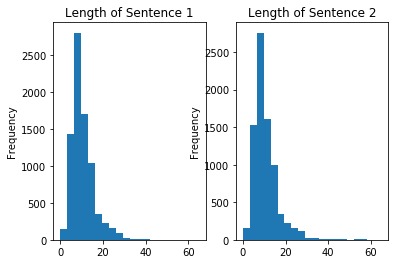
\includegraphics[width=0.48\textwidth]{fig/dist_sent_len.png} 
\caption{Distribution of sentence length: 8000 pairs from Quora dataset}
\end{figure}

\subsubsection{LSTM encoder}
Long Short Term Memory Network (LSTM) is first developed by Hochreiter and Schmidhuber \cite{hochreiter1997long}. Practically, a plain RNN has the problem of vanishing gradient and cannot capture long-dependencies when training over long sequences. However, Long Short Term Memory (LSTM) RNN addresses this problem by introducing a few gates which can control access to the cell state.

We briefly describe the idea of LSTM here \cite{colah2015lstm}. As illustrated in Figure 1, an LSTM memory cell consists of four layers:
\begin{figure}[htbp]
\centering
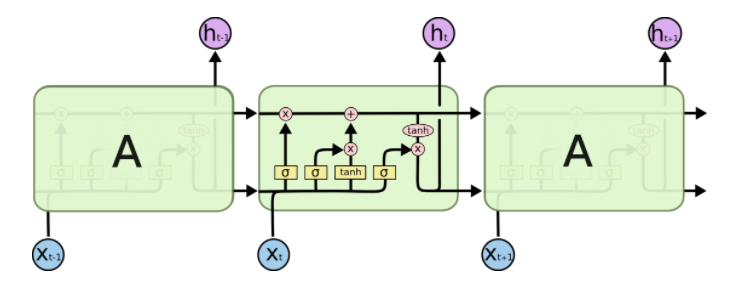
\includegraphics[width=0.48\textwidth]{fig/LSTM.png}
\caption{Illustration of LSTM}
%\caption*{Description}
\end{figure}
 
\begin{itemize}
    \item Forget gate: $f_t = \sigma(W_f\cdot[h_{t-1},x_t] +b_f)$, where input is current $x_t$ and previous output $h_{t-1}$. The output (an quantity between 0 and 1 for each number in cell state $C_{t-1}$) decides the probability of what information to keep.
    \item This layers contains two components. An input gate: $i_t = \sigma(W_i\cdot[h_{t-1},x_t] +b_i)$ decides which values to update. And a tanh layer: $\tilde{C}_t = tanh(W_C\cdot[h_{t-1},x_t] +b_C)$ which proposes a set of new candidates $\tilde{C}_t $
    \item Update cell state $C_{t} = f_t*C_{t-1} +i_t * \tilde{C_t}$, which basically means forgetting old information ($f_t*C_{t-1}$) and adding new information ($i_t * \tilde{C_t}$)
    \item Output gate: $o_t = \sigma(W_o\cdot[h_{t-1},x_t] +b_o)$ and $h_t = o_t * \tanh(C_t)$ which is a filtered cell state.
\end{itemize}

To implement LSTM encoders, the word embeddings will be fed into an LSTM model to generate sentence embedding. 

\section{Experiments}
We evaluate our model on a subset of the Quora question pairs dataset available on Kaggle, which is released by Quora and contains 8,000 lines of potential duplicate question pairs. Each line contains six columns: ID of the question pair, IDs for each question in the pair, the full text for each question, and a binary indicators which marks whether the two questions in the pair are duplicate. We use accuracy, precision, recall and F1 score as our evaluation metrics. The dataset is split to be: train 75 \%, development 15 \%, test 15 \%.

\subsection{Feature-rich classifier model}
We implemented sum of words embedding + random forest classifier as the baseline model. The performance over development data and test data are presented in Table 1 and 2. Using the same dataset which contains nearly 40k sentence pairs, the cross-unigram model performs the best among all in terms of F1-score, despite that they share almost the same score in terms of accuracy. We can safely draw the conclusion that the POS tagging knowledge helped improve the predicting of the logistic regression model used (logistic regression and random forest). For example, the premise "How can I be a good geologist?" and the hypothesis "What should I do to be a great geologist?", the ending tokens of these two sentences share the same POS tags (can: MODAL, should: MODAL; I: PRON; be: VERB; a: DET; good/great: ADJ; geologist: NOUN/entity!) and are counted as having a collection of cross-unigram features (should, I, be, a, great, geologist). The intuition comes from the fact that verb-noun phrases and potential modifiers (adjectives, adverbs) tend to decide the meaning of a sentence than other word categories. Thus it is essential to extract the main structure from the sentence, here, word embedding is one way, the number of dimensions used to represent a word also matters, here we tried the vector representation of 50 dimension and 100 dimension, respectively. Also, the cross-bigram model helps raise the recall rate, in the way that bigram is also an important and useful feature in text understanding. Besides, as sentence inversion is pretty common, in order to recognize such inverse structures, cross-bigram-inverse model is also used to measure how well this feature can be used to predict the most.

\begin{table}[h]
\begin{center}
\begin{tabular}{|l|llll|}
\hline Model &  Acc. & Prec. &  Recall & F1 \\ \hline
Baseline  & 0.64 & 0.55 & 0.28 & 0.37\\
Cross-unigram & 0.68 & 0.58 & 0.48 & 0.53\\
Cross-bigram & 0.66 & 0.56 & 0.33 & 0.42\\
inverse-bigram& 0.65 & 0.55 & 0.33 & 0.41\\
\hline
\end{tabular}
\end{center}
\caption{ Performance on development data}
\end{table}

\begin{table}[h]
\begin{center}
\begin{tabular}{|l|llll|}
\hline Model & Acc. & Prec.  & Recall & F1 \\ \hline
Baseline & 0.66 &  0.62 & 0.33 & 0.43 \\
Cross-unigram & 0.69 & 0.59 & 0.47 & 0.52 \\
Cross-bigram & 0.69 & 0.65 & 0.35 & 0.46 \\
inverse-bigram& 0.69 & 0.64 & 0.36 & 0.46\\
\hline
\end{tabular}
\end{center}
\caption{ Performance on test data}
\end{table}


\subsection{LSTM sentence embedding model}
All models are implemented in TensorFlow.  We use cross-entropy as the training objective. The models are trained using Adam Optimizer with stochastic minibatch. 
\paragraph{Tuning Hyper-parameters}  Choosing the right parameters is more of art than science. The methods for learning problem diagnosis and hyper-parameters tuning for our model refers to \cite{pompeyart}. In this paper, the hyper-parameters we focus on are:
\begin{itemize}
    \item Learning rate: The fixed learning rate we pass here is an initialization value. Adam optimizer will adjust the learning rate during the process of training.
    \item Dropout: dropout techniques are applied to all hidden layers of the neural network classifier and input and output of LSTM.
    \item $L_2$ regularization are applied to all models.
\end{itemize}

\paragraph{Results} Finally, we select a learning rate of 0.001, a dropout keep rate of 0.5  for both sum of words model and LSTM model. The $L_2$ regularization strength is set to be 0.01 for sum of words and 0.1 for LSTM. The accuracy for development and test data are presented in Table 3. We didn't find that LSTM has an obvious advantage over the baseline sum of words. This is partly due to the over-fitting problem. Because of speed issue, we just trained on 8000 pairs of data, which makes the Bowman's data-intensive method too complex for this dataset.

\begin{table}[h]
\begin{center}
\begin{tabular}{|l|rr|}
\hline\bf Accuracy & Dev & Test \\ \hline
SumOfWords & 0.63  & 0.63 \\
LSTM  & 0.65  &  0.61 \\
\hline 
\end{tabular}
\end{center}
\caption{Accuracy on dev and test dataset by different sentence model}
\end{table}

To compare the sentence embedding performance for the models, we also investigated the sentence representation vectors for some examples. For duplicate sentence pairs shown in table 4, LSTM encoders always give higher similarity measure. Especially for the second pair, which has less syntatic similarity, sum of words embedding gives relatively low similarity, while  LSTM still yield good result.

\begin{table}[ht]
	\begin{center}
		\begin{tabular}{lcc}
			\hline
			Sentence Pair & Sum & LSTM \\
			\hline
			\specialcell{How can I be a good geologist?}  & \multirow{2}{*}{ 0.9205} &  \multirow{2}{*}{\bf 0.9901} \\
			 \specialcell{What should I do to e a \\ great geologist?} & & \\
			\hline
			\specialcell{Astrology: I am a Capricorn Sun \\ Cap moon and cap rising...\\what does that say about me?}  & \multirow{2}{*}{ 0.8972} &  \multirow{2}{*}{\bf 0.9884} \\
			\specialcell{I'm a triple Capricorn (Sun, Moon  \\ and ascendant in Capricorn) \\ What does this say about me?} & & \\
			\hline
		\end{tabular}
	\end{center}
	\caption{Cosine Similarity for duplicate sentence pairs by two models}
\end{table}

\paragraph{Qualitative Error Analysis} Both models failed when the inference needs world knowledge and external resources. For example, for the duplicate sentence pair: \textit{How is the new Harry Potter book 'Harry Potter and the Cursed Child'?} and \textit{How bad is the new book by J.K Rowling?}, both models predict it as non-duplicate since the relationship between 'Harry Potter book' and 'J.K Rowling' cannot be inferred merely by the context. Thus, for the future work, we can consider incorporating external knowledge base and entity linking.  They also both failed to correctly predict non-duplicate questions when the sentences largely share lexical and syntactic information. For example:  \textit{What can be done to reduce the pollution of India?} and \textit{What is the best way to reduce pollution in india?}, are predicted as duplicate by both models. Most of the words are the same, and 'What can be done ' and 'What is the (best) way' are similar phrases. Attention model can potentially improve the prediction in this case, since it might will assign more attention weight to the word 'best'.

\section{Conclusions and Future Work}
In this paper, we implemented two models. One is feature-rich classifier model, which uses lexical and semantic information to build features such as cross-unigram, cross-bigram, inverse-bigram etc. We also implemented sentence embedding models based on sum of words and LSTM. All these methods outperform the baseline method.

 Our evaluation is based on a subset of the original data. We are planning to evaluate our current methods on the complete dataset (a large corpus), since data-intensive models are more practically important. 

Potential directions to improve current methods include but are not limited to: 
\begin{itemize}
    \item Implement batch normalization to alleviate LSTM over-fitting problem
    \item Improve the LSTM encoder by using bidirectional LSTM (biLSTM) to generate sentence embedding
    \item Implement lexical mapping and discover more promising features such as the mapping between acronyms and full names, named entity matching, etc.
\end{itemize}

% include your own bib file like this:
%\bibliographystyle{acl}
%\bibliography{acl2017}
\bibliography{project.bib}{}
\bibliographystyle{acl_natbib}

%\appendix

\end{document}
